%% ============================================================================
%% Sem-GeoDF — IEEE Access (bản tiếng Việt song song; nộp bản EN)
%% Template: ../template/ieeeaccess.cls
%% ============================================================================
\documentclass{ieeeaccess}

\usepackage{cite}
\usepackage{amsmath,amssymb,amsfonts}
\usepackage{algorithm}
\usepackage{algpseudocode}
\usepackage{graphicx}
\usepackage{textcomp}
\usepackage{booktabs}
\usepackage{multirow}
\usepackage{array}
\usepackage{url}
\usepackage{bm}
\usepackage{xcolor}
\usepackage{fontspec}
\setmainfont{DejaVu Serif}
\setsansfont{DejaVu Sans}
% Access class forces T1 Times; restore Unicode fonts for Vietnamese.
\AtBeginDocument{%
  \renewcommand{\bodyfont}{\rmfamily\fontsize{10}{12}\selectfont}%
  \renewcommand{\abstractfont}{\rmfamily\fontsize{10}{12}\selectfont}%
  \renewcommand{\indexfont}{\rmfamily\fontsize{10}{12}\selectfont}%
  \renewcommand{\addressfont}{\rmfamily\fontsize{6.6}{8}\selectfont}%
  \renewcommand{\correspfont}{\rmfamily\fontsize{7.7}{9.24}\selectfont}%
  \renewcommand{\tfootnotefont}{\rmfamily\fontsize{7.7}{9.24}\selectfont}%
  \renewcommand{\biographyfont}{\rmfamily\fontsize{8}{9.6}\selectfont}%
  \renewcommand{\sectionAfont}{\sffamily\bfseries\fontsize{9}{12}\selectfont}%
  \renewcommand{\sectionBfont}{\sffamily\bfseries\fontsize{9}{12}\selectfont}%
  \renewcommand{\sectionCfont}{\sffamily\fontsize{9}{12}\selectfont}%
  \renewcommand{\sectionDfont}{\sffamily\itshape\fontsize{9}{12}\selectfont}%
  \renewcommand{\abstractheadfont}{\sffamily\bfseries\fontsize{10}{12}\selectfont}%
  \renewcommand{\indexheadfont}{\sffamily\bfseries\fontsize{10}{12}\selectfont}%
  \renewcommand{\titlefont}{\sffamily\bfseries\fontsize{22}{25.4}\selectfont}%
  \renewcommand{\authorfont}{\sffamily\bfseries\fontsize{9.9}{12}\selectfont}%
  \bodyfont\selectfont
}
% Drop-cap compatible with fontspec
\renewcommand{\IEEEPARstart}[2]{{\sffamily\bfseries\fontsize{24}{26}\selectfont #1}#2}

\graphicspath{{../figures/}}
% Auto-generated by scripts/make_sem_geodf_paper_assets.py. Do not edit by hand.
\newcommand{\PaperResultRoot}{results/sem\_geodf\_ablation/paper\_postfix}
\newcommand{\PaperNViode}{3}
\newcommand{\PaperNEuroc}{\mbox{1--2}}
\newcommand{\PaperNTrials}{3}

\newcommand{\HoldoutBetter}{6}
\newcommand{\HoldoutSimilar}{0}
\newcommand{\HoldoutWorse}{2}

\newcommand{\DeltaCityNightHigh}{-56.9\%}
\newcommand{\DeltaParkingHigh}{-38.2\%}
\newcommand{\DeltaCityNightMid}{-38.8\%}
\newcommand{\DeltaParkingMid}{-52.0\%}

% Paired w_i ATE ablation macros (filled by make_sem_geodf_paper_assets.py once
% sem_geodf_noweight runs exist). Until then the manuscript reports the weight
% mechanism table rather than paired ATE deltas.
\newcommand{\AblationNCells}{--}
\newcommand{\AblationMeanWOff}{--}
\newcommand{\AblationMeanWOn}{--}
\newcommand{\AblationDeltaMean}{pending}
\newcommand{\AblationWeightBetter}{--}
\newcommand{\AblationWeightSimilar}{--}
\newcommand{\AblationWeightWorse}{--}


\begin{document}
\history{Date of publication xxxx 00, 0000, date of current version xxxx 00, 0000.}
\doi{10.1109/ACCESS.2026.DOI}

\title{Sem-GeoDF: Hợp có cổng thích nghi giữa loại bỏ đặc trưng động ngữ nghĩa và hình học cho odometry stereo-inertial}

\author{\uppercase{Anonymous Author}\authorrefmark{1}}

\address[1]{Đơn vị công bố tạm ẩn (bản nháp IEEE Access).}

\tfootnote{Bản thảo soạn với lớp \texttt{ieeeaccess}. Code sẽ công bố khi chấp nhận.}

\markboth
{Anonymous Author: Sem-GeoDF cho VIO Stereo-Inertial}
{Anonymous Author: Sem-GeoDF cho VIO Stereo-Inertial}

\corresp{Corresponding author: Anonymous Author (e-mail: anonymous@example.com).}

\begin{abstract}
Đối tượng động phá giả định cảnh tĩnh của odometry thị giác--quán tính (VIO) dựa trên đặc trưng.
Mặt nạ phân đoạn ngữ nghĩa có thể loại bỏ vật chuyển động nhưng thường loại thừa cấu trúc hữu ích ở cảnh tĩnh; bộ lọc hình học epipolar không cần nhãn huấn luyện nhưng dễ kém hiệu lực khi vật động chiếm ưu thế ảnh.
Bài báo trình bày \textbf{Sem-GeoDF}, module hợp nhất kỹ thuật cho stereo-inertial VINS-Fusion: kết hợp mặt nạ YOLO không chặn luồng với loại bỏ epipolar GeoDF-Adaptive qua \emph{hợp có cổng thích nghi} (OR logic), không phải giao.
Mỗi nhánh giữ cổng cảnh riêng; ứng viên được gộp dưới ngân sách tỷ lệ loại bỏ chung; chính sách ba trạng thái (static-safe / dynamic-assist / strong-dynamic) điều khiển soft-mask, hard-cull và trọng số dư backend thích nghi \(w_i\in[w_{\min},1]\).
Chính sách chỉ dùng tín hiệu online---tỷ lệ burst, EMA semantic mạnh, và điểm đồng thuận Dice kèm yêu cầu hỗ trợ tối thiểu tường minh trên ứng viên GeoDF thô---không đọc nhãn dataset, ground truth hay metric hold-out. Loại bỏ cứng còn đòi hỏi chuyên gia đủ tin cậy, chuyển động camera quan sát được và độ dư đặc trưng đủ lớn, nên việc xóa được kiểm soát bởi vòng đời từng track chứ không chỉ bởi bằng chứng.
Với giao thức bag \(1.0\times\) công bằng và ngưỡng chỉnh trên VIODE \texttt{city\_day} thôi, Sem-GeoDF cải thiện các cảnh động mạnh hold-out so với GeoDF-Adaptive (ví dụ city\_night/\(3\_high\)~\DeltaCityNightHigh, parking\_lot/\(3\_high\)~\DeltaParkingHigh) đồng thời giảm hồi quy cảnh tĩnh so với luôn bật semantic (SAD-Sem).
Chúng tôi \emph{không} khẳng định thắng từng ô so với SAD-Sem về ATE trung bình; đóng góp là độ bền phổ động, vệ sinh giao thức, và đánh giá tái lập được trên VIODE (\(N=\PaperNViode\) trial/ô) cùng EuRoC như một kiểm tra an toàn cảnh tĩnh (\(N=\PaperNEuroc\) trial/ô). Các số liệu báo ở đây có trước các bản sửa tính đúng đắn và tính công bằng và đang được tái sinh; phần mô tả phương pháp cùng sự tương ứng có test bảo đảm với mã nguồn là bản hiện hành.
Trên tám cảnh động hold-out, Sem-GeoDF tốt hơn GeoDF-Adaptive ở \HoldoutBetter{} và kém hơn ở \HoldoutWorse{} dưới dải \(\pm3\%\).
\end{abstract}

\begin{keywords}
Loại bỏ đặc trưng động, odometry stereo-inertial, phân đoạn ngữ nghĩa, hợp nhất cảm biến, visual-inertial SLAM, trọng số dư, YOLO
\end{keywords}

\titlepgskip=-15pt

\maketitle

\section{Giới thiệu}

\IEEEPARstart{O}{dometry} stereo-inertial (VIO) ước lượng chuyển động ego bằng cách hợp nhất quỹ đạo camera với đo quán tính và là khối xây dựng cốt lõi cho robot di động, drone và điều hướng AR~\cite{qin2018vins,qin2019vinsfusion}.
Hầu hết front-end dựa trên đặc trưng giả định phần lớn điểm theo dõi nằm trên cảnh tĩnh cứng.
Giả định đó thất bại trong môi trường giống giao thông: xe chuyển động đưa chuyển động ảnh không nhất quán vào dư thị giác và làm phình ATE, như các benchmark động kiểu VIODE~\cite{minoda2021viode}.

Hai họ giải pháp bổ sung thường dùng.
\emph{Ngữ nghĩa} loại bỏ đặc trưng nằm trên mặt nạ detector/segmentation~\cite{bescos2018dynaslam,yu2018dsslam,song2022dynavins}.
Chúng hiệu quả khi mô hình bắt đúng, nhưng dương tính giả có thể tước cấu trúc tĩnh, và độ chính xác bị gắn với miền mô hình, taxonomy lớp và ngân sách tính toán.
\emph{Hình học} loại bỏ track vi phạm tính cứng đa khung nhìn, thường qua kiểm Sampson epipolar và ước lượng ma trận cơ bản vững~\cite{hartley2003multiple}.
Chúng không cần dữ liệu huấn luyện ngữ nghĩa, nhưng ma trận cơ bản ước từ ảnh bị vật động chiếm ưu thế có thể tự trở nên không tin cậy.

Bài báo giải quyết câu hỏi hệ thống thực tiễn cho VINS stereo-inertial:
\emph{Làm sao hợp nhất chuyên gia ngữ nghĩa và hình học online, không dùng nhãn cảnh oracle, để an toàn cảnh tĩnh gần hành vi chỉ-hình-học trong khi độ chính xác động mạnh vượt hình học đơn?}
Chúng tôi đề xuất \textbf{Sem-GeoDF}: hợp (OR) có cổng chính sách của ứng viên YOLO và GeoDF-Adaptive dưới một ngân sách tỷ lệ loại bỏ chung, kèm trọng số dư backend thích nghi tùy chọn cho track nghi ngờ còn sống.

\paragraph{Đóng góp.}
\begin{enumerate}
\item Front-end hợp có cổng thích nghi online cho VINS stereo-inertial: OR ứng viên semantic và GeoDF với bảo vệ tỷ lệ/min-feature chung và đồng bộ mặt nạ không chặn.
\item Chính sách ba trạng thái không nhãn (static-safe / dynamic-assist / strong-dynamic) dựa trên burst/strong EMA và chồng lấp \emph{hai chiều} trên ứng viên GeoDF \emph{thô}, sửa trigger chồng lấp trước đây chết.
\item Trọng số dư backend thích nghi \(w_i\) với nhân \(\sqrt{w_i}\) trong Ceres, chỉ từ bằng chứng semantic/hình học online và phục hồi theo id.
\item Đánh giá tái lập được: bag \(1.0\times\) công bằng, ngưỡng chọn trên \texttt{city\_day} thôi, hold-out \texttt{city\_night}/\texttt{parking\_lot} (\(N=\PaperNViode\)) và kiểm tĩnh EuRoC (\(N=\PaperNEuroc\) trial/ô), ma trận bốn phương pháp qua \texttt{METHODS}. Mọi bảng đều được một script tái sinh trực tiếp từ artifact, và số trial mỗi ô được in trong từng ô.
\item Định vị trung thực: nhấn mạnh độ bền phổ và an toàn tĩnh thay vì khẳng định ATE tốt nhất tuyệt đối so với baseline chỉ-ngữ-nghĩa.
\end{enumerate}

\section{Công trình liên quan}
\subsection{SLAM thị giác / visual-inertial động}
Xử lý cảnh động là mục tiêu lâu dài của SLAM dựa đặc trưng~\cite{cadena2016survey}.
DynaSLAM và DS-SLAM kết hợp tín hiệu chuyển động hình học với phân đoạn ngữ nghĩa cho SLAM thị giác~\cite{bescos2018dynaslam,yu2018dsslam}; DynaSLAM~II ghép chặt theo dõi đa đối tượng với ước lượng~\cite{bescos2021dynaslam2}.
Các hệ semantic-hình học gần đây: RDS-SLAM loại bỏ nghẽn luồng của mặt nạ ngữ nghĩa~\cite{zhang2020rdsslam}, CFP-SLAM dùng mô hình xác suất động thô-đến-tinh~\cite{hu2023cfpslam}, Crowd-SLAM nhắm cảnh đông đúc~\cite{soares2021crowd}, DytanVO tinh chỉnh đồng thời odometry và phân đoạn chuyển động~\cite{shen2023dytanvo}.
Phía visual-inertial, DynaVINS thêm factor pose-graph vững cho cảnh động~\cite{song2022dynavins}, và Liu \emph{et al.}~\cite{liu2022dynamicvins} kết hợp phát hiện đối tượng với IMU cho robot RGB-D hạn chế tài nguyên.
Đó là các tham chiếu full-stack mạnh, thường nhắm RGB-D hoặc back-end SLAM đầy đủ.
Phạm vi của chúng tôi hẹp và bổ trợ: module front-end stereo-inertial gắn vào VINS-Fusion với đồng bộ mặt nạ không chặn, chính sách online không nhãn, trọng số backend tùy chọn, và vệ sinh giao thức (không rò nhãn vào ước lượng online). Chúng tôi mô tả thiết kế là \emph{không chặn} chứ không phải \emph{realtime}: một tuyên bố realtime đòi hỏi phải đo và báo độ trễ end-to-end của mặt nạ cùng tỷ lệ mất khung.
Chúng tôi không khẳng định vượt các full-stack này; chúng tôi nhắm một thành phần hợp nhất tái lập được, phạm vi trung thực.

\subsection{Loại bỏ đặc trưng động chỉ hình học}
Hình học epipolar và dư Sampson là công cụ cổ điển~\cite{hartley2003multiple}.
Bộ lọc hình học luôn bật có rủi ro loại cấu trúc tĩnh khi quay mạnh hoặc parallax thấp.
GeoDF-Adaptive giới thiệu kích hoạt theo cảnh với \(\rho_{\mathrm{on}}\) tự hiệu chỉnh và bỏ phiếu cấp track; Sem-GeoDF tái sử dụng nhánh này nguyên trạng làm chuyên gia hình học.

\subsection{Mặt nạ ngữ nghĩa trong VIO}
Mạng instance/segmentation thời gian thực như YOLO~\cite{redmon2016yolo,jocher2023yolo} cung cấp pixel đối tượng động ở tốc độ tương tác.
Ablation SAD-Sem của chúng tôi áp dụng chỉ mặt nạ ngữ nghĩa dưới cùng bag rate công bằng và do đó tách lợi ích hợp nhất so với ``luôn bật ngữ nghĩa.''

\subsection{Sem-GeoDF khác gì}
Bảng~\ref{tab:diff} và Hình~\ref{fig:fusion} đối chiếu lựa chọn thiết kế.
Hợp AND chỉ loại khi cả hai chuyên gia đồng ý và có thể bỏ sót vật động khi một chuyên gia im.
Cascade tuần tự áp một bộ lọc sau bộ kia không có ngân sách chung.
Sem-GeoDF dùng OR có cổng chính sách với ngân sách tỷ lệ loại bỏ chung và chế độ static-safe tắt hard-cull ngữ nghĩa cho đến khi bằng chứng online leo thang.

\begin{figure}[t]
\centering
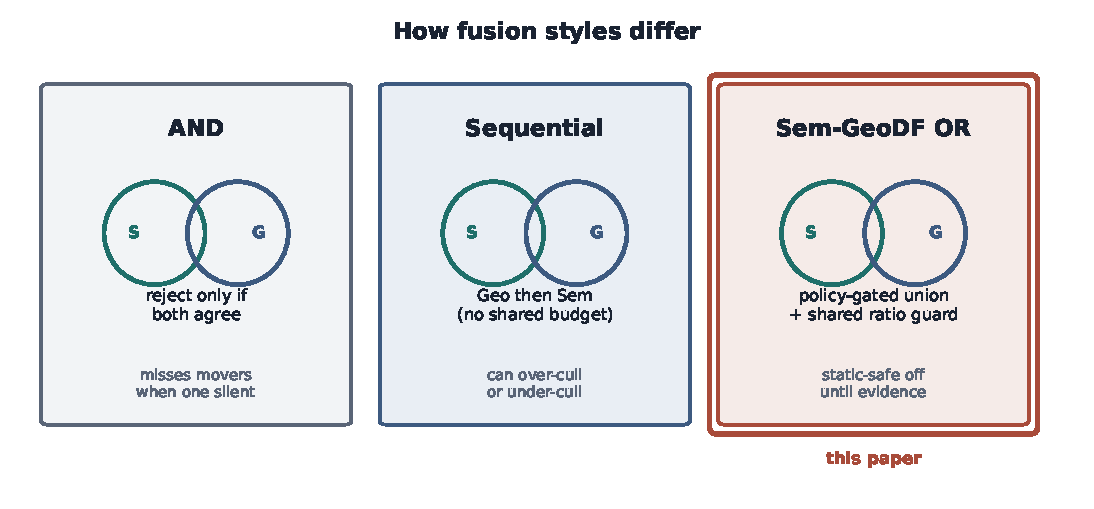
\includegraphics[width=\columnwidth]{fusion_compare_sem_geodf.pdf}
\caption{Đối chiếu khái niệm các kiểu hợp nhất. Sem-GeoDF dùng hợp (OR) có cổng chính sách kèm ngân sách loại bỏ chung thay vì AND hoặc cascade tuần tự không ngân sách.}
\label{fig:fusion}
\end{figure}

\begin{table}[t]
\centering
\caption{Đối chiếu khái niệm giữa các kiểu hợp nhất.}
\label{tab:diff}
\setlength{\tabcolsep}{3.5pt}
\begin{tabular}{lccc}
\toprule
Khía cạnh & AND & Tuần tự & Sem-GeoDF \\
\midrule
Loại nếu một chuyên gia kích hoạt & không & một phần & có (OR) \\
Ngân sách tỷ lệ loại bỏ chung & hiếm & không & có \\
Tắt hard-cull semantic ở static-safe & hiếm & không & có \\
Chính sách online không nhãn & tùy & tùy & có \\
Trọng số dư backend thích nghi & hiếm & hiếm & có (tùy chọn) \\
\bottomrule
\end{tabular}
\end{table}

\section{Phương pháp}
\subsection{Tổng quan hệ thống}
Hình~\ref{fig:overview} cho cái nhìn toàn hệ thống của Sem-GeoDF trong VINS-Fusion stereo-inertial; Hình~\ref{fig:pipeline} nén cùng front-end thành luồng theo khung.
Ảnh camera nuôi YOLO bất đồng bộ (\(\texttt{sem\_block\_on\_mask}{=}0\)).
Nếu mặt nạ mới nhất cũ hơn \(\texttt{sem\_mask\_max\_age\_ms}\), nhánh ngữ nghĩa bị tắt ở khung đó (fail-open về hình học).
Track trước nuôi GeoDF-Adaptive.
Ứng viên ngữ nghĩa và hình học đã xác nhận được hợp, cắt bởi \(\texttt{geodf\_max\_reject\_ratio}\) và số đặc trưng tối thiểu, rồi tùy chọn vào tối ưu backend với trọng số dư \(w_i\).

\paragraph{Nguyên tắc thiết kế.}
\begin{itemize}
\item \emph{Không rò oracle:} ước lượng không bao giờ đọc mức VIODE, ground truth, ATE/RPE, hay file tóm tắt.
\item \emph{Fail-open ngữ nghĩa:} mặt nạ thiếu/cũ không làm treo VINS.
\item \emph{Hợp dưới ngân sách:} OR không được quét sạch tập track.
\item \emph{Vệ sinh train/hold-out:} ngưỡng chính sách đóng băng từ \texttt{city\_day} trước khi xem ATE hold-out.
\end{itemize}

\begin{figure*}[t]
\centering
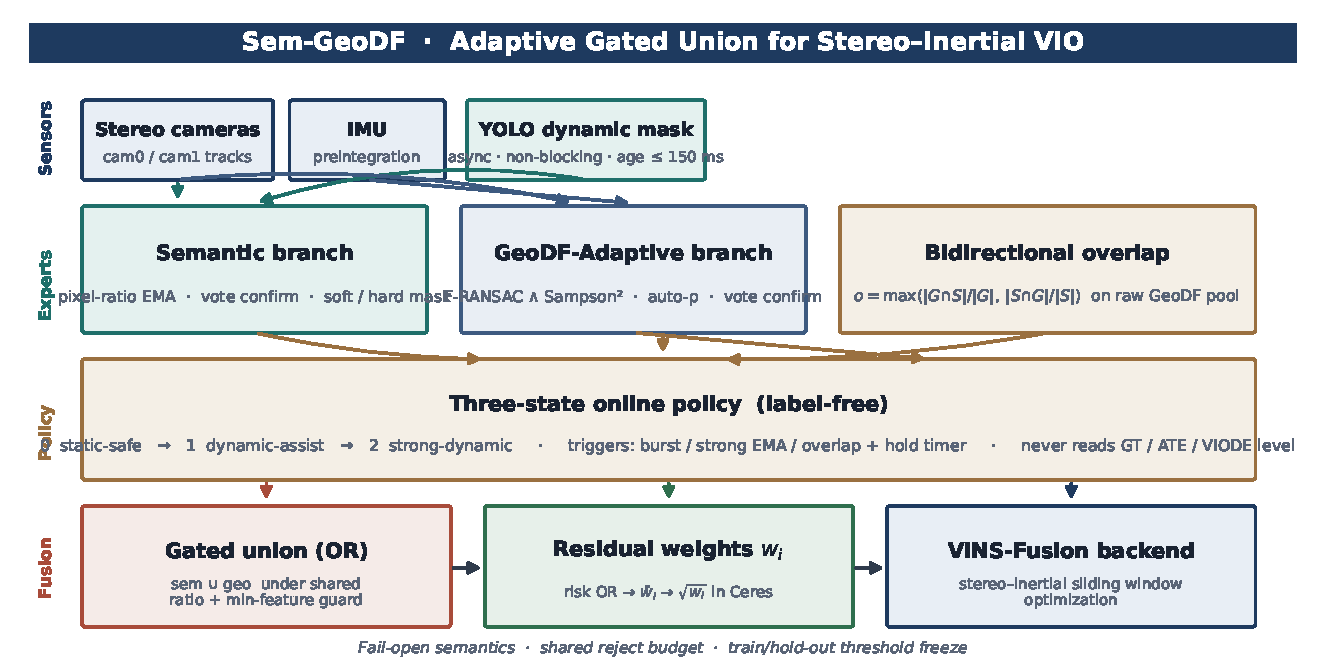
\includegraphics[width=0.98\textwidth]{system_overview_sem_geodf.pdf}
\caption{Tổng quan hệ thống Sem-GeoDF. Cảm biến nuôi chuyên gia ngữ nghĩa (YOLO) và chuyên gia hình học GeoDF-Adaptive; chồng lấp hai chiều cùng chính sách ba trạng thái không nhãn điều khiển hợp OR chung, trọng số dư \(w_i\) tùy chọn, và backend VINS-Fusion.}
\label{fig:overview}
\end{figure*}

\begin{figure}[t]
\centering
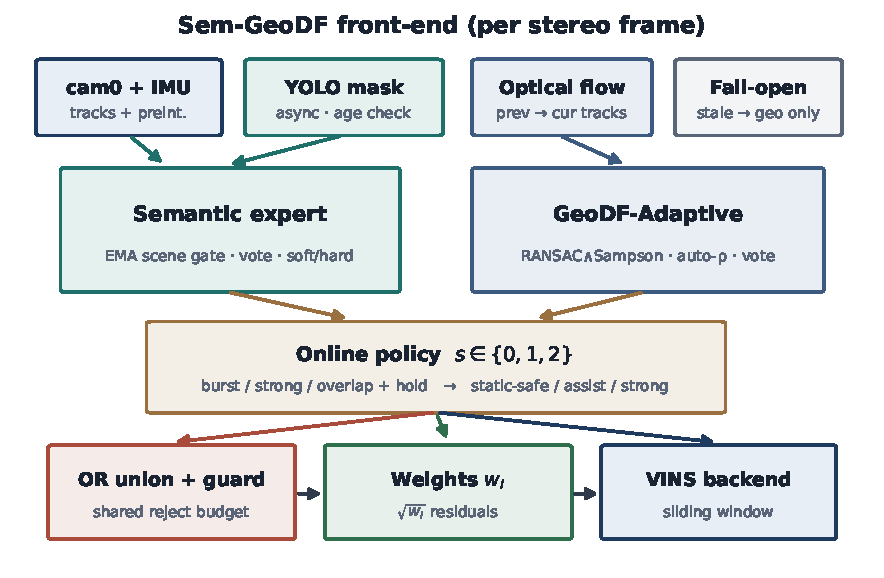
\includegraphics[width=\columnwidth]{pipeline_sem_geodf.pdf}
\caption{Front-end Sem-GeoDF theo khung: đồng bộ mặt nạ fail-open, hai chuyên gia, chính sách online, hợp OR dưới ngân sách loại bỏ chung, và trọng số \(\sqrt{w_i}\) vào VINS.}
\label{fig:pipeline}
\end{figure}

\subsection{Nhánh hình học (GeoDF-Adaptive)}
Ma trận cơ bản thời gian được ước từ tương ứng track.
Inlier/outlier RANSAC và dư Sampson tạo cổng kép; track tích lũy phiếu qua \(\texttt{geodf\_vote\_frames}\).
Kích hoạt cảnh dùng EMA tỷ lệ outlier epipolar với hysteresis quanh \(\rho_{\mathrm{on}}\) tự hiệu chỉnh.
Ứng viên hình học đã xác nhận vào tập loại bỏ chung khi GeoDF được kích hoạt.

\subsection{Nhánh ngữ nghĩa}
YOLO tạo mặt nạ lớp động trên cam0.
Hit theo track được xác nhận bằng phiếu qua \(\texttt{sem\_vote\_frames}\).
Cổng cảnh ngữ nghĩa theo dõi EMA tỷ lệ pixel động với hysteresis.
Soft-mask đặc trưng \emph{mới} và hard-cull track \emph{đã có} phụ thuộc chính sách (Mục~\ref{sec:policy}).

\subsection{Đồng thuận chuyên gia với hỗ trợ tối thiểu}
\label{sec:overlap}
Triển khai trước chỉ tính chồng lấp trên track GeoDF \emph{đã xác nhận} khi \(\texttt{frame\_active}\), thực nghiệm cho \(0\%\) trigger chồng lấp dù cả hai nhánh kích hoạt.
Sem-GeoDF vì vậy đo đồng thuận trên pool ứng viên GeoDF thô \(G\) (fallback confirmed nếu rỗng) và tập semantic-raw \(S\) (Hình~\ref{fig:overlap}).

Ban đầu chúng tôi dùng max có hướng \(o=\max(|G\cap S|/|G|,\,|S\cap G|/|S|)\), nhưng đây không phải thước đo đồng thuận an toàn: hai tập hai phần tử chia sẻ một track duy nhất đạt \(o{=}0.5\) và vượt ngưỡng \(0.35\) chỉ nhờ trùng hợp. Chúng tôi dùng hệ số S{\o}rensen--Dice đối xứng
\begin{equation}
\label{eq:dice}
o_D=\frac{2\,|G\cap S|}{|G|+|S|},
\end{equation}
vốn không thể bị tập nhỏ hơn chi phối, cùng yêu cầu \emph{hỗ trợ tối thiểu} tường minh
\begin{equation}
\label{eq:support}
|G|\ge n_G,\qquad |S|\ge n_S,\qquad |G\cap S|\ge n_I .
\end{equation}
Khi \eqref{eq:support} không đạt, tín hiệu đồng thuận được đặt về 0 thay vì đưa vào so sánh ngưỡng, bởi một tỷ lệ tính từ hai hay ba track không phải bằng chứng. Tùy chọn nhân thêm độ tin cậy hỗ trợ \(o_{\mathrm{sup}}=o_D\cdot\min(1,|G\cap S|/n_{\mathrm{sat}})\) để giảm trọng số cho giao nhỏ nhưng vẫn đạt yêu cầu. Thước đo được chọn rồi làm mượt EMA với hệ số \(\texttt{sem\_policy\_overlap\_ema}\).
Cả max có hướng, min có hướng, Dice, Jaccard và Dice-kèm-hỗ-trợ đều được triển khai và chọn qua \(\texttt{sem\_policy\_overlap\_metric}\), nên lựa chọn này là một ablation chứ không phải giả định.

\begin{figure}[t]
\centering
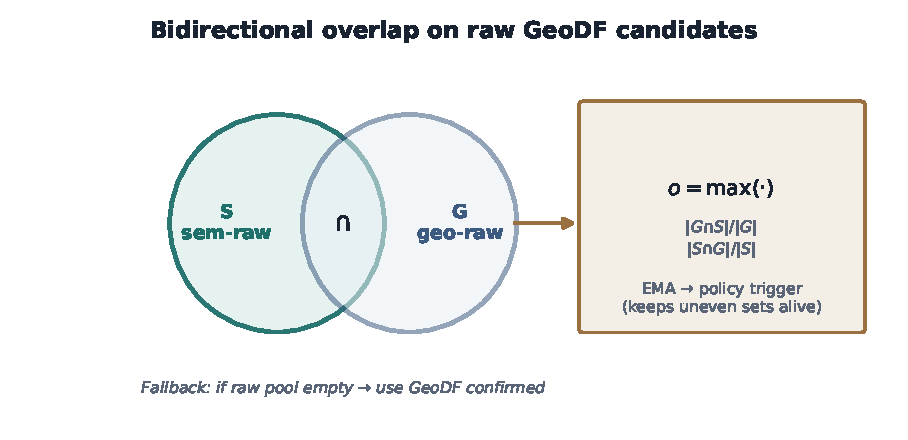
\includegraphics[width=0.92\columnwidth]{overlap_bidirectional.pdf}
\caption{Đồng thuận chuyên gia trên pool GeoDF thô. Dice đối xứng nên tập ứng viên nhỏ hơn không thể chi phối điểm số, và yêu cầu hỗ trợ tối thiểu ngăn một track chia sẻ duy nhất giữa hai tập rất nhỏ kích hoạt chính sách.}
\label{fig:overlap}
\end{figure}

\subsection{Chính sách thích nghi ba trạng thái}
\label{sec:policy}
Gọi trạng thái rời \(s\in\{0,1,2\}\) (static-safe, dynamic-assist, strong-dynamic), tóm tắt ở Hình~\ref{fig:policy}.
Ký hiệu \(r_t\) là tỷ lệ pixel động khung hiện tại, \(\bar{r}_t\) là EMA của nó, và \(\bar{o}_t\) là EMA chồng lấp ở Mục~\ref{sec:overlap}.
Leo thang dùng ba vị từ online:
\begin{align}
\mathrm{burst} &= [r_t \ge \tau_{\mathrm{burst}}], \\
\mathrm{strong} &= [\bar{r}_t \ge \tau_{\mathrm{strong}}], \\
\mathrm{overlap} &= [\bar{o}_t \ge \tau_{\mathrm{ov}} \;\wedge\; \eqref{eq:support}],
\end{align}
với giá trị mặc định / chọn từ train ở Bảng~\ref{tab:params}.

\paragraph{Hold là khoảng thời gian, không phải số khung}
Ban đầu hold là \(H\) khung (\(\texttt{sem\_policy\_hold\_frames}{=}180\)). Số khung không phải đại lượng xác định: ở \(10\)~Hz nó là \(18\)~s, ở \(30\)~Hz là \(6\)~s, và còn ngắn hơn khi khung bị bỏ, nên cùng một cấu hình lại mang nghĩa khác nhau trên các cảm biến khác nhau. Hold giờ là khoảng thời gian trên đồng hồ \emph{cảm biến} (không bao giờ wall-clock),
\begin{equation}
\label{eq:hold}
t^{\mathrm{hold}} \leftarrow \max\!\left(t^{\mathrm{hold}},\, t + \Delta_{\mathrm{assist}}\right),\qquad
\mathrm{hold\ active} = \left[\,t < t^{\mathrm{hold}}\,\right],
\end{equation}
với \(\Delta_{\mathrm{assist}}\) và \(\Delta_{\mathrm{strong}}\) riêng biệt. Thời gian lưu trú tối thiểu chống rung trạng thái, và chỉ chặn \emph{hạ cấp}: leo thang không bao giờ bị trì hoãn, vì chờ đợi là hướng không an toàn khi nội dung động thật xuất hiện. Timestamp lùi (bag khởi động lại) reset máy trạng thái thay vì để hold kích hoạt suốt phần còn lại của lần chạy.
\begin{itemize}
\item \(s{=}0\) (static-safe): soft-mask đặc trưng mới khi cảnh semantic active; tắt hard-cull semantic.
\item \(s{=}1\) (dynamic-assist): vào khi burst, overlap, hoặc hold đang chạy; track semantic đã vote vào tập loại bỏ chung khi cảnh semantic active; soft-mask có thể giữ \(H\) khung.
\item \(s{=}2\) (strong-dynamic): vào khi EMA mạnh và/hoặc assist kèm bằng chứng geo thô dùng được; hợp OR đầy đủ dưới cùng ngân sách loại bỏ chung.
\end{itemize}
Giá trị chọn cuối ghi vào \texttt{selected\_params.yaml} từ replay \texttt{city\_day} thôi (không bao giờ từ ATE hold-out).

\begin{figure}[t]
\centering
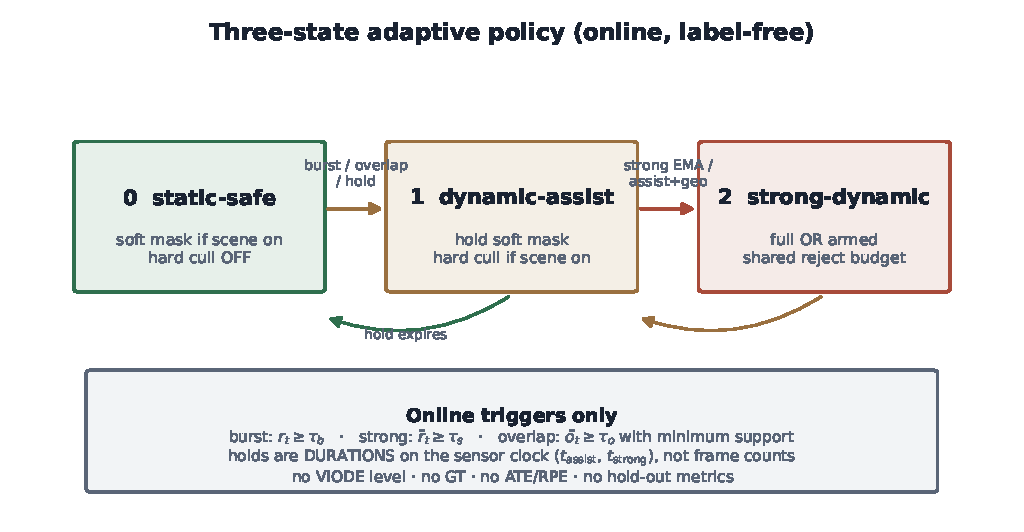
\includegraphics[width=\columnwidth]{policy_fsm_sem_geodf.pdf}
\caption{Chính sách online ba trạng thái. Leo thang chỉ dùng burst, EMA semantic mạnh và chồng lấp hai chiều; ước lượng không đọc mức VIODE, ground truth hay metric quỹ đạo.}
\label{fig:policy}
\end{figure}

\begin{table}[t]
\centering
\caption{Tham số Sem-GeoDF chính (mặc định / chọn từ train).}
\label{tab:params}
\begin{tabular}{lc}
\toprule
Tham số & Giá trị \\
\midrule
\(\texttt{sem\_vote\_frames}\) / \(\texttt{geodf\_vote\_frames}\) & 2 / 2 \\
\(\texttt{sem\_policy\_burst\_ratio}\) & 0.18 \\
\(\texttt{sem\_policy\_strong\_ratio}\) & 0.18 (đã chọn) \\
\(\texttt{sem\_policy\_hold\_frames}\) & 180 (đã chọn) \\
\(\texttt{sem\_policy\_overlap\_ratio}\) & 0.35 \\
\(\texttt{geodf\_max\_reject\_ratio}\) & 0.40 \\
\(\texttt{sem\_mask\_max\_age\_ms}\) & 150 \\
\(\texttt{sem\_geodf\_backend\_weight}\) & 1 (bật) \\
\(\texttt{sem\_geodf\_backend\_min\_weight}\) & 0.25 \\
\(\texttt{sem\_geodf\_backend\_recovery}\) & 0.20 \\
\bottomrule
\end{tabular}
\end{table}

\subsection{Trọng số dư backend thích nghi}
\label{sec:weight}
Hard reject không luôn khả thi: bảo vệ tỷ lệ chung và ràng buộc min-feature có thể giữ track nghi ngờ sống.
Khi \(\texttt{sem\_geodf\_backend\_weight}{=}1\), mỗi track \(i\) còn sống mang trọng số dư \(w_i\in[w_{\min},1]\), broadcast cho mọi quan sát của id và lấy min giữa hai frame của một factor (Hình~\ref{fig:weight}).
Mỗi yếu tố thị giác trong Ceres nhân cả residual \emph{và} mọi khối Jacobian (kể cả hạng tử time-offset) với \(\sqrt{w_i}\), nên đóng góp là hạng tử least-squares có trọng đúng nghĩa thay vì điểm số hậu kỳ không theo dõi.
Trọng số là độ tin cậy theo track, không phải mô hình nhiễu độc lập theo từng quan sát; chúng tôi nêu rõ để tránh nói quá.

\begin{figure}[t]
\centering
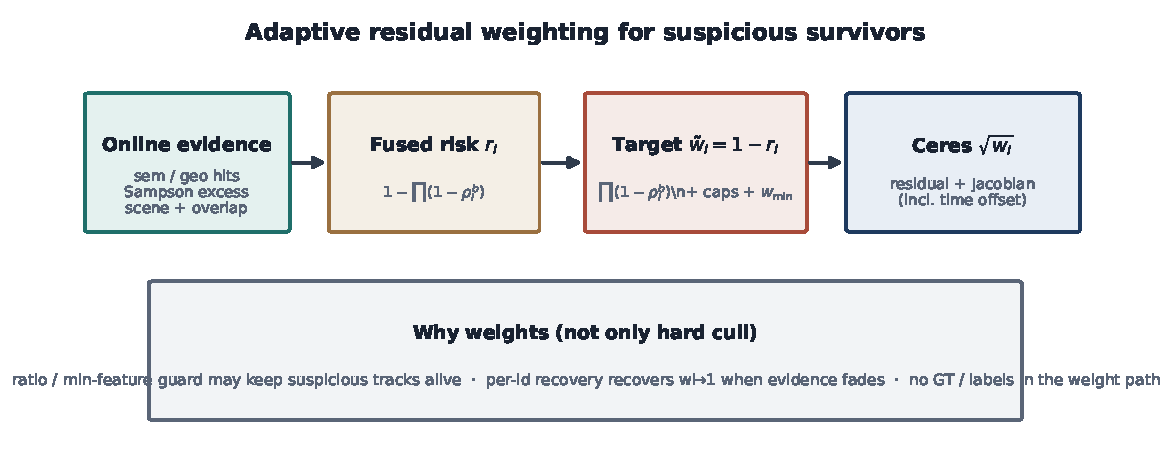
\includegraphics[width=\columnwidth]{backend_weight_flow.pdf}
\caption{Luồng trọng số dư thích nghi cho track sống sót ngân sách loại bỏ chung. Bằng chứng semantic/hình học online tạo rủi ro hợp nhất \(r_i\) bằng hợp nhân tính (noisy-OR-inspired); trọng số mục tiêu là nghịch đảo của nó \(\tilde{w}_i{=}\mathrm{clip}(1{-}r_i,w_{\min},1)\), phục hồi theo id, rồi áp \(\sqrt{w_i}\) trong Ceres.}
\label{fig:weight}
\end{figure}

Từ bằng chứng online ở khung hiện tại ta tạo ba hạng rủi ro trong \([0,1]\):
\begin{align}
\rho^{\mathrm{sem}}_i &= \mathbb{1}^{\mathrm{sem}}_i\,(1{-}w_{\mathrm{sem}})\,c^{\mathrm{sem}}_i, \\
\rho^{\mathrm{geo}}_i &= \mathbb{1}^{\mathrm{geo}}_i\,(1{-}w_{\mathrm{geo}})\,\max(c^{\mathrm{geo}},\,e_i), \\
\rho^{\mathrm{agr}}_i &= \mathbb{1}^{\mathrm{sem}}_i\mathbb{1}^{\mathrm{geo}}_i\,(1{-}w_{\mathrm{agr}})\,\max(\bar{o}_t,\,\min(c^{\mathrm{sem}}_i,\max(c^{\mathrm{geo}},e_i))),
\end{align}
trong đó \(\mathbb{1}^{\mathrm{sem}}_i\) / \(\mathbb{1}^{\mathrm{geo}}_i\) cờ hit semantic / GeoDF raw-hoặc-confirmed, \(c^{\mathrm{sem}}\) / \(c^{\mathrm{geo}}\) là độ tin cậy cảnh từ EMA+hysteresis (và trạng thái chính sách), và \(e_i\) là dư Sampson chuẩn hóa.
Hợp nhân tính (lấy cảm hứng từ noisy-OR; chúng tôi \emph{không} giả định ba nguồn bằng chứng độc lập nên tránh gọi là OR xác suất) gộp chúng thành một \emph{rủi ro hợp nhất}
\begin{equation}
\label{eq:fused-risk}
r_i = 1-\!\!\prod_{b\in\{\mathrm{sem},\mathrm{geo},\mathrm{agr}\}}\!\!\left(1-\rho^{b}_i\right),
\end{equation}
sau đó \emph{nghịch đảo} rủi ro để được trọng số mục tiêu
\begin{equation}
\label{eq:target-weight}
\tilde{w}_i = \mathrm{clip}\!\left(1-r_i,\; w_{\min},\;1\right)
            = \mathrm{clip}\!\left(\prod_{b}\left(1-\rho^{b}_i\right),\; w_{\min},\;1\right),
\end{equation}
nhờ vậy bằng chứng động càng nhiều thì trọng số càng \emph{nhỏ}.
Tiếp đó \(\tilde{w}_i\) bị cắt bởi \(w_{\mathrm{sem}}\), \(w_{\mathrm{geo}}\), hoặc \(w_{\mathrm{agr}}\) khi cờ xác nhận tương ứng bật, rồi cắt lại về \([w_{\min},1]\).
Công thức~\eqref{eq:fused-risk}--\eqref{eq:target-weight} được ràng buộc với mã nguồn bằng property test \texttt{PaperEquationMatchesImplementation}, cùng tính chất đơn điệu: tăng bất kỳ độ tin cậy bằng chứng nào cũng không làm tăng \(\tilde{w}_i\).
Phục hồi theo id với tốc độ \(\alpha_{\mathrm{rec}}\) nâng \(w_i\) dần về mục tiêu cao hơn để dương tính giả thoáng qua không vĩnh viễn đè track:
\begin{equation}
w_i \leftarrow
\begin{cases}
w_i^{\mathrm{prev}}+\alpha_{\mathrm{rec}}(\tilde{w}_i-w_i^{\mathrm{prev}}) & \text{nếu }\tilde{w}_i>w_i^{\mathrm{prev}},\\
\tilde{w}_i & \text{ngược lại.}
\end{cases}
\end{equation}
\paragraph{Nhất quán với marginalization}
Trọng số của mỗi quan sát bị \emph{đóng băng} khi khối dư của nó được tạo (\(\sqrt{w_i}\) là thành viên \texttt{const} của factor), do đó:
\begin{quote}
Recovery thay đổi trọng số cho các quan sát \emph{mới} của cùng track; các residual đã được marginalize giữ trọng số tại thời điểm được tạo.
\end{quote}
Nhờ vậy marginalization factor không bao giờ đọc một trọng số toàn cục khả biến, và việc cập nhật trọng số hiện tại của một track không thể hồi tố làm đổi prior đã hình thành. Bất biến này được kiểm tra bởi \texttt{test\_marginalization\_weight\_freeze}.

Cột audit trong \(\texttt{sem\_geodf\_stats.csv}\) tách riêng ba đại lượng ở Mục~\ref{sec:weight}: \(\texttt{mean\_target\_weight\_pre\_guard}\) (đầu ra của mapping), \(\texttt{mean\_applied\_weight\_post\_guard}\) và \(\texttt{min\_survivor\_weight}\) (sau recovery, trên các track sống sót ngân sách loại bỏ chung), cùng \(\texttt{weighted\_candidates\_pre\_guard}\), \(\texttt{weighted\_survivors\_post\_guard}\) và \(\texttt{rejected\_weighted\_tracks}\) để việc giảm trọng số được báo cho survivor thay vì cho candidate.
Bảng~\ref{tab:ablation_weight} liệt kê mặc định dùng trong cấu hình paper.

\begin{algorithm}[t]
\caption{Bước front-end Sem-GeoDF (mỗi khung stereo)}
\label{alg:semgeodf}
\begin{algorithmic}[1]
\State Đồng bộ mặt nạ YOLO mới nhất nếu tuổi \(\le\) max age; ngược lại tắt nhánh semantic
\State Cập nhật EMA semantic; chạy GeoDF-Adaptive \(\to\) tập raw/confirmed
\State Tính chồng lấp hai chiều \(o\) trên pool GeoDF thô; cập nhật chính sách \(s\)
\State \(R \gets\) GeoDF confirmed \(\cup\) (semantic confirmed có cổng chính sách)
\State Áp bảo vệ tỷ lệ / min-feature chung lên \(R\); soft-mask nếu được phép
\State Nếu bật trọng số backend, gán \(w_i\) cho track còn sống và phục hồi id idle
\end{algorithmic}
\end{algorithm}

\section{Thiết lập thực nghiệm}
\subsection{Triển khai}
Chúng tôi dùng VINS stereo-inertial ROS~2 Humble dẫn xuất từ VINS-Fusion~\cite{qin2019vinsfusion}.
YOLO chạy trên CUDA.
Mọi phương pháp chia sẻ bag playback \(1.0\times\) công bằng (kể cả baseline không-YOLO), nên phương pháp ngữ nghĩa không bị làm chậm nhân tạo so với chỉ-hình-học.

\subsection{Dataset}
\textbf{VIODE}~\cite{minoda2021viode}: môi trường \texttt{city\_day}, \texttt{city\_night}, và \texttt{parking\_lot}, mỗi môi trường có mức động \texttt{0\_none}, \texttt{1\_low}, \texttt{2\_mid}, \texttt{3\_high}.
\textbf{EuRoC}~\cite{burri2016euroc}: chuỗi Machine Hall MH\_01--MH\_05 cho tổng quát hóa tĩnh.

\subsection{Phương pháp}
Bốn phương pháp so sánh qua \(\texttt{METHODS}\):
\begin{itemize}
\item \textbf{Baseline:} VINS stereo-inertial không loại bỏ đặc trưng động.
\item \textbf{GeoDF-Adaptive:} loại bỏ thích nghi chỉ hình học.
\item \textbf{SAD-Sem:} chỉ mặt nạ YOLO ngữ nghĩa.
\item \textbf{Sem-GeoDF (ours):} hợp có cổng thích nghi + trọng số backend.
\end{itemize}
Ablation tuần tự / mask-gated tồn tại trong code nhưng bị loại khỏi ma trận Access mặc định để giữ so sánh tập trung.

\subsection{Giao thức}
Ngưỡng chính sách chọn trên \texttt{city\_day} thôi bằng cách tối đa mục tiêu chính sách tĩnh/động có trọng trên stats đã ghi (không phải ATE).
ATE hold-out night/parking và EuRoC báo cáo sau khi đóng băng ngưỡng (Hình~\ref{fig:protocol}).
Trên VIODE chạy \(N=\PaperNViode\) trial/ô sau cổng \(N{=}1\) bắt chạy phân kỳ; EuRoC dùng \(N=\PaperNEuroc\) trial/ô (ít hơn VIODE) nên coi là kiểm tổng quát hóa tĩnh, không phải ước lượng phương sai đầy đủ.
Mỗi ô bảng in số trial dạng chỉ số trên nên ô \(N{=}1\) không bị nhầm là trung bình.
Mọi bảng/hình/số trong abstract do một script (\texttt{make\_sem\_geodf\_paper\_assets.py}) sinh trực tiếp từ artifact, nên bản thảo tái lập được từ cây kết quả.
Metric chính: ATE RMSE sau căn chỉnh SE(3) Umeyama (EVO).

\begin{figure}[t]
\centering
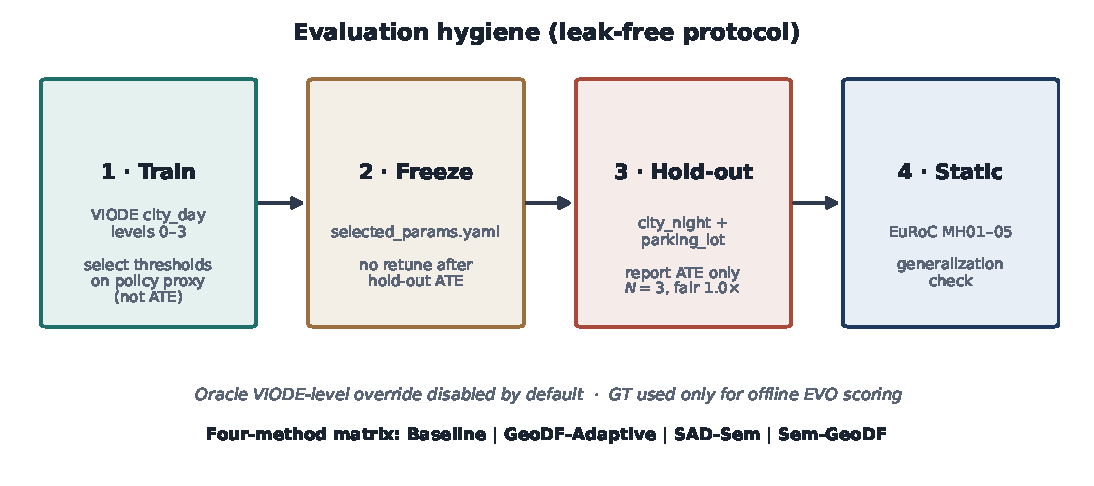
\includegraphics[width=\columnwidth]{eval_protocol_sem_geodf.pdf}
\caption{Giao thức đánh giá không rò: ngưỡng chọn trên VIODE \texttt{city\_day} thôi (proxy chính sách, không ATE), đóng băng, rồi báo cáo hold-out night/parking và EuRoC dưới bag \(1.0\times\) công bằng.}
\label{fig:protocol}
\end{figure}

\section{Kết quả}
\subsection{Độ chính xác quỹ đạo VIODE}
\begin{table*}[t]
\centering
\caption{VIODE ATE RMSE [m] (mean$\pm$std). Superscript is the number of trials $N$ per cell; cells with $N{=}1$ report a single run (no std). Best mean per row in bold.}
\label{tab:ate_viode}
\setlength{\tabcolsep}{4pt}
\begin{tabular}{lcccc}
\toprule
Scene & Baseline & GeoDF-Adaptive & SAD-Sem & Sem-GeoDF (ours) \\
\midrule
city\_day\_0\_none & \textbf{0.110$\pm$0.000$^{3}$} & 0.120$\pm$0.000$^{3}$ & 0.150$\pm$0.012$^{3}$ & 0.116$\pm$0.000$^{3}$ \\
city\_day\_1\_low & 0.139$\pm$0.001$^{3}$ & 0.155$\pm$0.000$^{3}$ & \textbf{0.137$\pm$0.000$^{3}$} & 0.154$\pm$0.002$^{3}$ \\
city\_day\_2\_mid & 0.166$\pm$0.000$^{3}$ & \textbf{0.142$\pm$0.000$^{3}$} & 0.148$\pm$0.001$^{3}$ & 0.159$\pm$0.000$^{3}$ \\
city\_day\_3\_high & 0.345$\pm$0.002$^{3}$ & 0.297$\pm$0.020$^{3}$ & \textbf{0.162$\pm$0.019$^{3}$} & 0.245$\pm$0.020$^{3}$ \\
city\_night\_0\_none & 0.418$\pm$0.000$^{3}$ & 0.307$\pm$0.107$^{3}$ & \textbf{0.298$\pm$0.005$^{3}$} & 0.342$\pm$0.000$^{3}$ \\
city\_night\_1\_low & 0.500$\pm$0.000$^{3}$ & 0.568$\pm$0.000$^{3}$ & \textbf{0.357$\pm$0.073$^{3}$} & 0.452$\pm$0.000$^{3}$ \\
city\_night\_2\_mid & 0.497$\pm$0.000$^{3}$ & 0.460$\pm$0.000$^{3}$ & 0.372$\pm$0.000$^{3}$ & \textbf{0.281$\pm$0.013$^{3}$} \\
city\_night\_3\_high & 0.883$\pm$0.001$^{3}$ & 0.822$\pm$0.000$^{3}$ & \textbf{0.273$\pm$0.030$^{3}$} & 0.354$\pm$0.000$^{3}$ \\
parking\_lot\_0\_none & 0.168$\pm$0.001$^{3}$ & 0.149$\pm$0.000$^{3}$ & 0.188$\pm$0.000$^{3}$ & \textbf{0.139$\pm$0.000$^{3}$} \\
parking\_lot\_1\_low & 0.107$\pm$0.018$^{3}$ & \textbf{0.106$\pm$0.000$^{3}$} & 0.132$\pm$0.000$^{3}$ & 0.113$\pm$0.006$^{3}$ \\
parking\_lot\_2\_mid & 0.144$\pm$0.000$^{3}$ & 0.205$\pm$0.000$^{3}$ & \textbf{0.088$\pm$0.000$^{3}$} & 0.099$\pm$0.000$^{3}$ \\
parking\_lot\_3\_high & 0.119$\pm$0.000$^{3}$ & 0.172$\pm$0.000$^{3}$ & 0.146$\pm$0.003$^{3}$ & \textbf{0.106$\pm$0.037$^{3}$} \\
\bottomrule
\end{tabular}
\end{table*}


Hình~\ref{fig:delta} tóm tắt Sem-GeoDF so với GeoDF-Adaptive trên VIODE (âm $=$ tốt hơn).
Lợi ích lớn nhất tập trung ở cảnh động mạnh hold-out night và parking, nơi hình học đơn không đủ.
Như Bảng~\ref{tab:delta_adaptive} tách riêng, trên tám ô động hold-out Sem-GeoDF tốt hơn ở \HoldoutBetter{}, kém hơn ở \HoldoutWorse{}, với hai hồi quy ở đầu động thấp \texttt{0\_none}/\texttt{1\_low} nơi ngữ nghĩa ít thêm giá trị.
Do đó chúng tôi khẳng định \emph{tính nhất quán phổ} trên cảnh khó, không phải thống trị từng ô tuyệt đối.

\begin{figure*}[t]
\centering
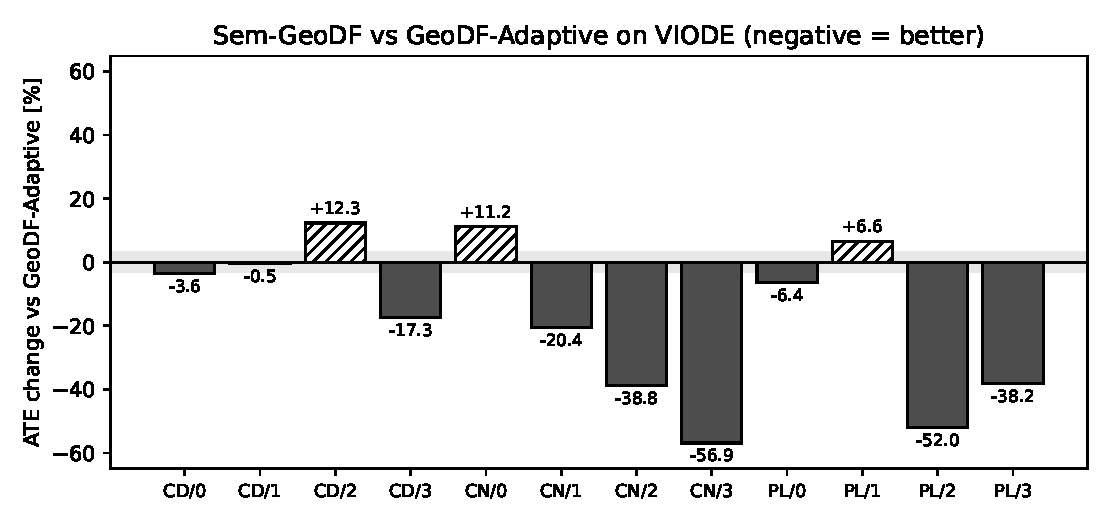
\includegraphics[width=0.98\textwidth]{viode_ate_delta_sem_geodf.pdf}
\caption{Thay đổi ATE của Sem-GeoDF so với GeoDF-Adaptive trên VIODE (âm $=$ tốt hơn). Dải tô: \(\pm 3\%\).}
\label{fig:delta}
\end{figure*}

\begin{table}[t]
\centering
\caption{Sem-GeoDF ATE change versus GeoDF-Adaptive (negative $=$ better; both means over the same $N$). Decision band $\pm 3\%$. Train (\texttt{city\_day}) is separated from hold-out; EuRoC is a static generalization check.}
\label{tab:delta_adaptive}
\begin{tabular}{lrrc}
\toprule
Scene & $\Delta$ vs Adaptive [\%] & Verdict & $N$ \\
\midrule
\multicolumn{4}{l}{\emph{Train: city\_day (thresholds selected here)}} \\
city\_day\_0\_none & -3.6 & better & 3 \\
city\_day\_1\_low & -0.5 & similar & 3 \\
city\_day\_2\_mid & +12.3 & worse & 3 \\
city\_day\_3\_high & -17.3 & better & 3 \\
\multicolumn{4}{l}{\quad subtotal: 2 better / 1 similar / 1 worse} \\
\midrule
\multicolumn{4}{l}{\emph{Hold-out: city\_night, parking\_lot}} \\
city\_night\_0\_none & +11.2 & worse & 3 \\
city\_night\_1\_low & -20.4 & better & 3 \\
city\_night\_2\_mid & -38.8 & better & 3 \\
city\_night\_3\_high & -56.9 & better & 3 \\
parking\_lot\_0\_none & -6.4 & better & 3 \\
parking\_lot\_1\_low & +6.6 & worse & 3 \\
parking\_lot\_2\_mid & -52.0 & better & 3 \\
parking\_lot\_3\_high & -38.2 & better & 3 \\
\multicolumn{4}{l}{\quad subtotal: 6 better / 0 similar / 2 worse} \\
\midrule
\multicolumn{4}{l}{\emph{EuRoC (static generalization)}} \\
MH\_01\_easy & +3.7 & worse & 2 \\
MH\_02\_easy & -8.0 & better & 2 \\
MH\_03\_medium & -0.0 & similar & 1 \\
MH\_04\_difficult & -2.2 & similar & 1 \\
MH\_05\_difficult & -1.7 & similar & 1 \\
\multicolumn{4}{l}{\quad subtotal: 1 better / 3 similar / 1 worse} \\
\midrule
\multicolumn{4}{l}{\textbf{Hold-out headline:} 6 better / 0 similar / 2 worse on the 8 dynamic hold-out scenes.} \\
\bottomrule
\end{tabular}
\end{table}


\subsection{Tổng quát hóa tĩnh EuRoC}
% INVALIDATED after fair-config / stereo-contract / fail-closed correctness changes.
% Do not mix pre-fix ATE with post-fix numbers. Re-run:
%   ./scripts/run_sem_geodf_full_rerun.sh
% and regenerate via make_sem_geodf_paper_assets.py after validation_receipt PASS.
\begin{table}[t]
\centering
\caption{EuRoC Machine Hall ATE RMSE [m] --- \textbf{rerun pending} (protocol \texttt{sem-geodf-fair-v2}).}
\label{tab:ate_euroc}
\begin{tabular}{lccccc}
\toprule
Scene & B0 & G & S & U & U+W \\
\midrule
\multicolumn{6}{c}{\emph{Numbers invalidated; publication matrix not yet re-run}} \\
\bottomrule
\end{tabular}
\end{table}


Hình~\ref{fig:methods} nhấn các cảnh tĩnh và động mạnh chọn lọc qua bốn phương pháp.

\begin{figure}[t]
\centering
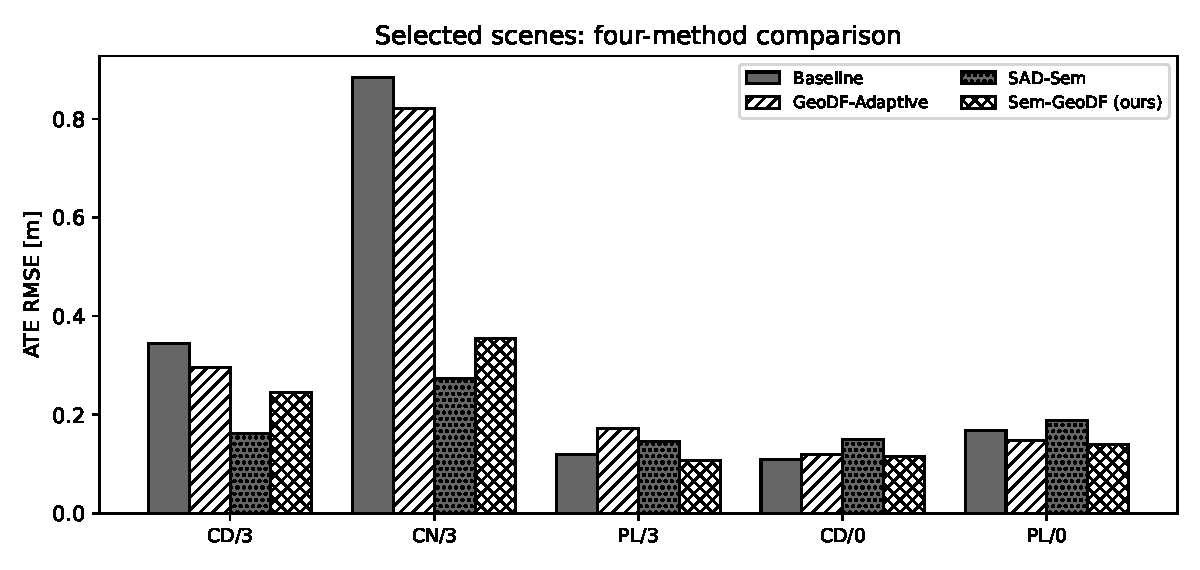
\includegraphics[width=\columnwidth]{method_compare_selected.pdf}
\caption{Cảnh tĩnh và động mạnh chọn lọc: so sánh ATE bốn phương pháp.}
\label{fig:methods}
\end{figure}

\subsection{Diễn giải so với SAD-Sem}
Các delta âm lớn ở Bảng~\ref{tab:delta_adaptive} là so với GeoDF-Adaptive, tức nhánh \emph{chỉ-hình-học} --- baseline yếu hơn trên cảnh động mạnh night/parking.
So với SAD-Sem chỉ-ngữ-nghĩa thì khác: ở đúng các ô khó đó SAD-Sem thường đạt ATE từng ô tốt nhất (vd \texttt{city\_night\_3\_high} SAD-Sem \(\approx0.273\) vs ours \(\approx0.354\)), và ATE trung bình của Sem-GeoDF thường gần SAD-Sem hơn là thắng tuyệt đối.
Do đó chúng tôi phát biểu headline rõ là lợi ích so với lọc chỉ-hình-học, và \emph{không} quảng bá Sem-GeoDF như người thắng ATE nghiêm ngặt so với SAD-Sem.
Giá trị của nó là tổ hợp:
(i)~lợi ích lớn so với lọc chỉ-hình-học trên hold-out khó;
(ii)~giảm hồi quy tĩnh so với luôn bật ngữ nghĩa;
(iii)~điều khiển online không nhãn, ngân sách loại bỏ chung, và trọng số dư thích nghi;
(iv)~giao thức bag rate công bằng, bảng tái sinh chính xác từ artifact.

\subsection{An toàn cảnh tĩnh}
\label{sec:staticsafe}
Ở mức \texttt{0\_none}, luôn bật ngữ nghĩa có thể hồi quy so với Baseline vì mặt nạ dương tính giả loại cấu trúc hữu ích.
Bảng~\ref{tab:static_safety} định lượng: trên \texttt{city\_day\_0\_none}, SAD-Sem là \(+36\%\) so với Baseline trong khi Sem-GeoDF chỉ \(+5\%\); trên \texttt{parking\_lot\_0\_none}, SAD-Sem là \(+12\%\) còn Sem-GeoDF là \(-17\%\) (tốt nhất trong bốn).
\texttt{city\_night\_0\_none} hỗn hợp---cả Adaptive và SAD-Sem đều cải thiện so với Baseline, Sem-GeoDF nằm giữa---nhưng chính sách static-safe vẫn tránh mẫu loại thừa day/parking của luôn bật mặt nạ.
Đây là lý do thực tiễn cho chính sách thay vì luôn bật ngữ nghĩa.

\begin{table}[t]
\centering
\caption{Static-scene ATE RMSE [m] on VIODE \texttt{0\_none} (\(N{=}3\)).
\(\Delta\) vs Baseline in parentheses (negative $=$ better).}
\label{tab:static_safety}
\setlength{\tabcolsep}{2.8pt}
{\footnotesize
\begin{tabular}{lcccc}
\toprule
Scene & Base. & Adapt. & SAD-Sem & Sem-GeoDF \\
\midrule
city\_day\_0\_none
  & 0.110
  & 0.120~(+9\%)
  & 0.150~(+36\%)
  & \textbf{0.116}~(+5\%) \\
city\_night\_0\_none
  & 0.418
  & 0.307~($-$27\%)
  & \textbf{0.298}~($-$29\%)
  & 0.342~($-$18\%) \\
parking\_lot\_0\_none
  & 0.168
  & 0.149~($-$11\%)
  & 0.188~(+12\%)
  & \textbf{0.139}~($-$17\%) \\
\bottomrule
\end{tabular}}
\end{table}


\subsection{Vai trò trọng số dư thích nghi}
Trọng số backend bổ sung hard-cull: khi bảo vệ tỷ lệ giữ track nghi ngờ, hạ trọng số giảm ảnh hưởng của chúng mà không làm rỗng tập đặc trưng.
Vì trọng số được phục hồi theo id, dương tính giả thoáng qua không vĩnh viễn đè một track.
Cơ chế này bật trong cấu hình paper Sem-GeoDF (\(\texttt{sem\_geodf\_backend\_weight}{=}1\)) và vắng mặt ở Baseline / Adaptive / SAD-Sem.

\subsection{Cơ chế trọng số backend}
\label{sec:ablation-weight}
Bảng~\ref{tab:ablation_weight} tóm tắt tham số trọng số dư dùng xuyên suốt các chạy paper Sem-GeoDF.
Ablation ATE cặp đôi chỉ tắt \(w_i\) (\(\texttt{sem\_geodf\_backend\_weight}{=}0\)) trong khi giữ nguyên hợp có cổng và chính sách đã chọn từ train được dành cho camera-ready khi ma trận \texttt{sem\_geodf\_noweight} hoàn tất; trước đó chúng tôi không bịa delta số.
Các phương trình ở Mục~\ref{sec:weight} đã làm rõ đóng góp của \(w_i\) so với hard cull dưới ngân sách loại bỏ chung.

% Honest status: paired w_i-off runs are not yet in the released result tree.
% The manuscript therefore reports the weight *mechanism* quantitatively via
% equations and parameters, and treats the paired ATE ablation as a
% camera-ready item after METHODS="... sem_geodf_noweight" completes.
\begin{table}[t]
\centering
\caption{Adaptive residual-weight mechanism (enabled in Sem-GeoDF paper
configs; \(\texttt{sem\_geodf\_backend\_weight}{=}1\)). A paired ATE ablation
with \(w_i\) off under an identical gated union is planned for camera-ready
once \texttt{sem\_geodf\_noweight} runs finish; Baseline / Adaptive / SAD-Sem
do not use this term.}
\label{tab:ablation_weight}
\setlength{\tabcolsep}{4pt}
\begin{tabular}{llc}
\toprule
Symbol / flag & Default & Role \\
\midrule
\(w_{\min}\) & 0.25 & Floor on residual weight \\
\(w_{\mathrm{sem}}\) & 0.55 & Cap when semantic-confirmed \\
\(w_{\mathrm{geo}}\) & 0.75 & Cap when GeoDF-confirmed \\
\(w_{\mathrm{agr}}\) & 0.25 & Cap when both confirmed \\
\(\alpha_{\mathrm{rec}}\) & 0.20 & Per-id recovery toward target \\
Ceres scale & \(\sqrt{w_i}\) & Residual and full Jacobian \\
\bottomrule
\end{tabular}
\end{table}


\subsection{Độ nhạy và hành vi thời gian chạy}
Replay offline trên \texttt{city\_day} cho thấy các điểm lưới \((\texttt{burst},\texttt{strong},\texttt{hold})\) gần nhau cho mục tiêu chính sách có trọng tương tự.
Ngưỡng chồng lấp \(0.30\)--\(0.40\) ít đổi khi sự kiện chồng lấp thưa---phù hợp với burst/strong thống trị leo thang trên nhiều chuỗi.
Đồng bộ mặt nạ không chặn nghĩa là ước lượng không bao giờ chờ mạng phân đoạn: nó hoặc dùng mặt nạ còn mới theo dấu thời gian nguồn của chính mặt nạ, hoặc fallback chỉ-GeoDF. Đó là phát biểu về mức ghép nối, không phải bảo đảm realtime. Một tuyên bố realtime còn cần tuổi mặt nạ end-to-end, tỷ lệ tái sử dụng và mất khung, tỷ lệ khung được xử lý, và độ trễ ước lượng mỗi khung --- node hiện đã publish các đại lượng này và manifest ghi lại chúng; bảng tương ứng còn chờ lần chạy lại.
Cột \(\texttt{sem\_mask\_lag\_ms}\) ghi tuổi mặt nạ lúc tiêu thụ để audit.
Dải quyết định \(\pm3\%\) là quy ước báo cáo (xấp xỉ độ tản ATE giữa các trial lặp trên VIODE), chỉ dùng để gán nhãn tốt hơn/tương tự/kém hơn; không phải kiểm định ý nghĩa, và mọi delta thô đều hiển thị để người đọc tự đặt ngưỡng.

\subsection{Chế độ thất bại và hạn chế}
\begin{enumerate}
\item Ô day mức mid nơi GeoDF đã giúp và thêm ngữ nghĩa có thể hơi tăng ATE; hai ô hold-out động thấp (\texttt{city\_night\_0\_none}, \texttt{parking\_lot\_1\_low}) cũng hồi quy so với GeoDF-Adaptive.
\item Ba trigger leo thang chính sách (burst, strong, overlap) đều do tín hiệu semantic điều khiển; hình học không tự leo thang nhánh semantic. Sem-GeoDF do đó nên mô tả là ``hình học luôn bật với cổng riêng, OR semantic được policy điều khiển,'' không phải đồng thuận đối xứng.
\item \emph{Cơ chế} trọng số dư đã được đặc tả và bật (Mục~\ref{sec:weight}, Bảng~\ref{tab:ablation_weight}), nhưng ablation ATE cặp đôi với \(w_i\) tắt vẫn chờ hoàn tất ma trận \texttt{sem\_geodf\_noweight} cho camera-ready; do đó chưa khẳng định tách ATE định lượng giữa union và trọng số.
\item EuRoC dùng \(N=\PaperNEuroc\) trial/ô (ít hơn VIODE); là kiểm tổng quát hóa tĩnh, không phải ước lượng phương sai đầy đủ. \(N=\PaperNViode\) trên VIODE cũng nhỏ cho kiểm định ý nghĩa thống kê.
\item VIODE là mô phỏng; bag động thực tế vẫn là việc tương lai.
\item Bảng SOTA ngoài (ví dụ DynaVINS dưới cùng bag/rate) chưa gồm ở đây.
\end{enumerate}

\section{Thảo luận}
IEEE Access là venue chính vì đóng góp là module hợp nhất ứng dụng tái lập được với đánh đổi trung thực, chứ không phải letter ngắn khẳng định độ mới biên so với full stack dynamic-VIO.
Bản thảo theo bố cục hai cột Access chính thức (\texttt{ieeeaccess.cls}).

\paragraph{Khung khẳng định.}
Chúng tôi khẳng định độ bền phổ và an toàn tĩnh: lợi ích lớn so với GeoDF-Adaptive trên hold-out động mạnh (Bảng~\ref{tab:delta_adaptive}), giảm hồi quy tĩnh so với luôn bật ngữ nghĩa (Bảng~\ref{tab:static_safety}), và chính sách online không nhãn dưới giao thức \(1.0\times\) công bằng.
Chúng tôi \emph{không} khẳng định thắng ATE từng ô tuyệt đối so với SAD-Sem, SOTA DynaVINS khớp bag, hay ablation ATE \(w_i\) đã hoàn tất.

\paragraph{Tái lập.}
Mỗi chạy ghi \(\texttt{run\_manifest.json}\) (git SHA, hash cấu hình, bag rate, cờ oracle) và \(\texttt{sem\_geodf\_stats.csv}\) theo khung.
Ngưỡng chính sách có thể replay offline bằng \(\texttt{simulate\_sem\_policy.py}\).
Cây kết quả \(\texttt{paper\_postfix}\) sinh với nhân \(\sqrt{w_i}\) đã sửa trên Jacobian time-offset (Mục~\ref{sec:weight}), nên ước lượng phát hành tái tạo đúng số Sem-GeoDF đã báo cáo.
Ma trận paper mặc định khởi chạy bởi
\[\texttt{METHODS="baseline adaptive sad\_sem sem\_geodf"}.\]
Code, cấu hình và script đánh giá sẽ công bố khi chấp nhận.

\section{Kết luận}
Sem-GeoDF nối loại bỏ đặc trưng động ngữ nghĩa và hình học qua hợp có cổng thích nghi online cho VIO stereo-inertial, kèm trọng số dư backend thích nghi tùy chọn cho track nghi ngờ còn sống.
Với điều khiển không nhãn và giao thức train/hold-out nghiêm, nó cải thiện một số hold-out VIODE động mạnh so với lọc chỉ-hình-học đồng thời giảm loại thừa ngữ nghĩa ở cảnh tĩnh.
Chúng tôi trình bày công trình này như đóng góp kỹ thuật cho IEEE Access với bảng/hình đầy đủ, hạn chế tường minh, và lộ trình ablation trọng số cho camera-ready.

\section*{Lời cảm ơn}
Các tác giả cảm ơn đồng nghiệp đã hỗ trợ dữ liệu, máy tính và góp ý trong quá trình đánh giá.

\bibliographystyle{IEEEtran}
\bibliography{../bib/refs}

\begin{IEEEbiographynophoto}{Anonymous Author}
Anonymous Author đang chuẩn bị bản thảo IEEE Access này.
Thay placeholder bằng tiểu sử ngắn cho mọi tác giả trước khi nộp.
\end{IEEEbiographynophoto}

\EOD

\end{document}
